\documentclass[10pt, a4paper, italian]{article}
\usepackage[T1]{fontenc}
\usepackage[utf8]{inputenc}
\usepackage{amsmath, amssymb, amsthm, thmtools, amsfonts, mathtools}
\usepackage{nicefrac}
\usepackage{calc}
\usepackage[pdftex, hyperindex, plainpages=false]{hyperref}
\usepackage[nameinlink]{cleveref} %load before classicthesis (clash)
%\usepackage[nochapters,pdfspacing]{classicthesis}
\usepackage{siunitx}
\usepackage[siunitx]{circuitikz}

\usepackage[a4paper]{geometry}
\usepackage{float}
\usepackage{mdframed}
\usepackage{titling}
\usepackage{booktabs}
\usepackage{graphicx}
\usepackage{caption, subcaption}
\usepackage{xcolor}
\usepackage[italian]{babel}
\usepackage{pgfplots}
\usepackage{listings}
%\usepackage{lmodern}
\usepackage{url}
\usepackage{enumitem}
\usepackage{tikz} %loads after classicthesis (xcolor incompat)

% lets graphicx know path where figures to be included are found
\graphicspath{{../figs/}}
\makeatletter
\def\input@path{{../figs/}}
%or: \def\input@path{{/path/to/folder/}{/path/to/other/folder/}}
\makeatother

% tikz pgf plots setup
\usepgfplotslibrary{external}
\pgfplotsset{compat=1.15}
%\tikzexternalize

% spaces and significant digits/figures for measurements
\sisetup{free-standing-units, space-before-unit, number-unit-product = \;,
scientific-notation = false, round-mode = figures, round-precision = 1,}

% turns all (hyperlinked) references black [default is blue]
\hypersetup{
	linktoc=all,
	colorlinks=true,
	linkcolor=black
}

% code listings config
%\lstset{
%language=Python,
%basicstyle=\ttfamily,
%columns=fullflexible,
%keepspaces=true,
%}

% mdframed (for boxed text) configuration
\mdfsetup{linewidth=0.6pt}

% Default fixed font does not support bold face
\DeclareFixedFont{\ttb}{T1}{txtt}{bx}{n}{12} % for bold
\DeclareFixedFont{\ttm}{T1}{txtt}{m}{n}{12}  % for normal

% Custom colors
\usepackage{color}
\definecolor{deepblue}{rgb}{0,0,0.5}
\definecolor{deepred}{rgb}{0.6,0,0}
\definecolor{deepgreen}{rgb}{0,0.5,0}

% Commands 
\newcommand{\executeiffilenewer}[3]{%
	\ifnum\pdfstrcmp{\pdffilemoddate{#1}}%
		{\pdffilemoddate{#2}}>0%
	{\immediate\write18{#3}}\fi%
}
% input .svg --> .pdf_tex graphs
%\newcommand{\includesvg}[1]{%
%	\executeiffilenewer{#1.svg}{#1.pdf}%
%	{inkscape -z -D --file=#1.svg %
%	--export-pdf=#1.pdf --export-latex}%
%	\input{#1.pdf_tex}%
%}
% Thanks UniPi's Department of Physics E. Fermi
\newcommand{\thanksdf}{(\thanks{Dipartimento di Fisica E.~Fermi,%
Universit\`a di Pisa - Pisa, Italy.}\;)}

% hyperlink to email address
\newcommand{\mail}[1]{\href{mailto:#1}{\textsf{#1}}}

% \vec for bold vectors, instead of overarrows (now "\arrvec")
\let\arrvec=\vec
\renewcommand{\vec}[1]{\boldsymbol #1}
% replaces straight phi with slanted phi
\renewcommand{\phi}{\varphi}
% replaces straight eps with curved epsilon
\newcommand{\eps}{\varepsilon}
% abbreviation for (sub_/super^)scripts of \lim, \sum,... in inline math
\newcommand{\ds}{\displaystyle}

% blackboard/number set letters
\newcommand{\CC}{\mathbb C}
\newcommand{\HH}{\mathbb H}
\newcommand{\KK}{\mathbb K}
\newcommand{\NN}{\mathbb N}
\newcommand{\PP}{\mathbb P}
\newcommand{\QQ}{\mathbb Q}
\newcommand{\RR}{\mathbb R}
\newcommand{\ZZ}{\mathbb Z}

\newcommand{\Abs}[1]{{\left\Vert #1\right\Vert}}
\newcommand{\enclose}[1]{{\left( #1 \right)}}
\newcommand{\Enclose}[1]{{\left[ #1 \right]}}
\newcommand{\floor}[1]{\left\lfloor #1 \right\rfloor}
\newcommand{\ceil}[1]{\left\lceil #1 \right\rceil}
\newcommand{\To}{\rightrightarrows}

% Math operators
\DeclareMathOperator{\divergence}{div}
\renewcommand{\div}{\divergence}
\DeclareMathOperator{\Imaginarypart}{Im}
\renewcommand{\Im}{\Imaginarypart}
\DeclareMathOperator{\Realpart}{Re}
\renewcommand{\Re}{\Realpart}
%\DeclareMathOperator{\arg}{arg}
\DeclareMathOperator{\tg}{tg}
\DeclareMathOperator{\arctg}{arctg}
\DeclareMathOperator{\settsinh}{settsinh}
\DeclareMathOperator{\settcosh}{settcosh}
\DeclareMathOperator{\tr}{tr}
\DeclareMathOperator{\im}{im}
\DeclareMathOperator{\sgn}{sgn}
\DeclareMathOperator{\diag}{diag}

\DeclarePairedDelimiter{\norm}{\lVert}{\rVert}
\DeclarePairedDelimiter{\scalar}{\langle}{\rangle}

% Logarithm with arbitrary base.
% -> log_10
\newcommand{\llog}[1][10]{\log_{#1}}

% Absolute value.
% -> |x|
\newcommand{\abs}[1]{\left| #1 \right|}

% Powers.
% -> x^a
\newcommand{\power}[2][2]{\left( #2 \right)^{#1}}

% Square.
% -> x^2
\newcommand{\sq}[1]{\power[2]{#1}}

% Expansion of the binomial coefficient.
% -> n1!/(n2!(n1 - n2)!)
\newcommand{\binomexpr}[2]{\frac{#1!}{#2!(#1 - #2)!}}

% Expression evaluation at a given point with square brackets.
% -> [x]_{a}
\newcommand{\at}[2]{\left[ #1\right]_{\makebox[-1pt][l]{${\scriptstyle#2}$}}}

% Expression evaluation in an interval.
% -> [x] _{a}^{b}
\newcommand{\eval}[3]{\left.#1%
  \right|_{\makebox[-1pt][l]{${\scriptstyle#2}$}}^{\makebox[-1pt][l]{${\scriptstyle#3}$}}}

% Upright d in math mode (for differentials).
% -> d
\newcommand{\ud}{\mathrm{d}}

% Differential.
% -> dx
\newcommand{\diff}[1][x]{\,\ud{#1}}

% Base command for defining derivatives.
% -> df/dx or d^kf/dx^k
\newcommand{\basederivative}[4][]{%
  \displaystyle%
  \ifx\\#1\\\frac{#4#2}{#4#3}%
  \else%
  \frac{#4^#1#2}{#4#3^#1}%
  \fi%
}

% Total derivative.
% -> df/dx(x) or d^kf/dx^k(x)
\newcommand{\td}[4][]{%
  \basederivative[#1]{#2}{#3}{\ud}%
  \ifx\\#4\\%
  \else%
  \mkern-4mu\left(#4\right)%
  \fi%
}

% Partial derivative.
% -> df/dx(x) or d^kf/dx^k(x)
\newcommand{\pd}[4][]{%
  \basederivative[#1]{#2}{#3}{\partial}%
  \ifx\\#4\\%
  \else%
  \mkern-4mu\left(#4\right)%
  \fi%
}

\newcommand{\intinf}{\int_{-\infty}^{\infty}\!\!\!}

\newcommand{\cinterval}[2]{\left[\, #1,~#2 \,\right]}

\newcommand{\linterval}[2]{\left[\, #1,~#2 \,\right)}

\newcommand{\rinterval}[2]{\left(\, #1,~#2 \,\right]}

\newcommand{\ointerval}[2]{\left(\, #1,~#2 \,\right)}

\newcommand{\prob}[1]{\displaystyle P\left(#1\right)}

\newcommand{\pvalue}{\emph{$p$-value}}

\newcommand{\cond}{\,|\,}

\newcommand{\expect}[1]{\displaystyle E\left[#1\right]}

\newcommand{\mom}[2][]{\displaystyle {\cal M}_{#2}\ifx\\#1\\\else(#1)\fi}

\newcommand{\momalg}[1]{\displaystyle \lambda_{#1}}

\newcommand{\momcen}[1]{\displaystyle \mu_{#1}}

\newcommand{\skewness}{\displaystyle \gamma_1}

\newcommand{\kurtosis}{\displaystyle \gamma_2}

\newcommand{\charf}[1][x]{\phi_{#1}}

\newcommand{\momgenf}[1][x]{M_{#1}}

\newcommand{\fwhm}{{\scriptstyle \textsc{FWHM}}}

\newcommand{\hwhm}{{\scriptstyle \textsc{HWHM}}}

\newcommand{\median}{\mu_{\nicefrac{1}{2}}}

\newcommand{\var}[1]{\ensuremath{\text{Var}\left(#1\right)}}

\newcommand{\cov}[2]{\ensuremath{\text{Cov}\left(#1, #2\right)}}

\newcommand{\corr}[2]{\ensuremath{\text{Corr}\left(#1, #2\right)}}

\newcommand{\like}{\mathcal L}

\newcommand{\likelihood}[2][]{\like\ifx\\#2\\\else(#2\ifx\\#1\\\else;#1\fi)\fi}

\newcommand{\chisq}{\ensuremath{\chi^2}}

\newcommand{\chisquare}[2][]{\chisq\ifx\\#2\\\else(#2\ifx\\#1\\\else;#1\fi)\fi}

\newcommand{\loglikelihood}[2][]{\log\likelihood[#1]{#2}}

\newcommand{\pdf}[3][]{#2(#3\ifx\\#1\\\else;#1\fi)}

\newcommand{\binomialpdf}[2][]{\pdf[#1]{\mathcal B}{#2}}

\newcommand{\multinomialpdf}[2][]{\pdf[#1]{\mathcal M}{#2}}

\newcommand{\poissonpdf}[2][]{\pdf[#1]{\mathcal P}{#2}}

\newcommand{\uniformpdf}[2][]{\pdf[#1]{u}{#2}}

\newcommand{\exponentialpdf}[2][]{\pdf[#1]{\varepsilon}{#2}}

\newcommand{\gausspdf}[2][]{\pdf[#1]{N}{#2}}

\newcommand{\chisquarepdf}[2][]{\pdf[#1]{\wp}{#2}}

\newcommand{\cauchypdf}[2][]{\pdf[#1]{c}{#2}}

\newcommand{\erf}[1]{\ensuremath{\text{erf}\left(#1\right)}}

\newcommand{\dccases}[4][]{#2 \ifx\\#2\\\else=\fi %
  \begin{cases}
    \displaystyle #3 & \text{per variabili discrete}\\
    \displaystyle #4 & \text{per variabili continue}#1
  \end{cases}
}
% sub/super-scriptable for all symbol as math operator 
\newcommand\Scaleforall[1]{\vcenter{\hbox{\scalefont{#1}$\forall$}}}

\DeclareMathOperator*\forevery{%
  \vphantom\sum
  \mathchoice{\Scaleforall{2}}{\Scaleforall{1.4}}{\Scaleforall{1}}{\Scaleforall{0.75}}}
\geometry{left=2cm, right=2cm, top=2cm, bottom=2cm}
\usepackage{svg}
% makes all hyperlinks the same color as text
\hypersetup{
	linktoc=all,
	colorlinks=false,
	linkcolor=black
	}
% lets graphicx know path where figures to be included are found
\graphicspath{{../figs/}}

\author{Gruppo 1.AC \\ Matteo Rossi, Bernardo Tomelleri}
\title{Es10: Misura del rapporto carica-massa dell'elettrone $e/m_e$}
\begin{document}
\date{\today}
\maketitle

%=======================
\section{Scopo dell'esperienza}
Si vuole misurare il rapporto $e/m$ attraverso la misura del raggio di
curvatura della traiettoria circolare di un fascio di elettroni immersi in un
campo magnetico uniforme (generato da bobine in configurazione di Helmholtz)
accelerati da una differenza di potenziale nota.

\section{Metodo di misura}
Consideriamo il campo magnetico prodotto da due bobine coassiali di raggio
medio $r = 15.8 \; \si{c\m}$, costituite da $N = 130$ spire collegate in
serie e percorse da una stessa corrente di intensità $I\ped{coil}$ da noi
controllabile.

Si può calcolare il campo magnetico nella regione vicino al centro di ciascuna
bobina dalla legge di Biot-Savart e, quando queste sono poste ad una distanza
$a = r$ pari al loro raggio -cioè in configurazione di Helmholtz- si può
ricavare un'espressione per il campo totale come sovrapposizione dei due campi
\begin{equation}\label{eq: B-helm}
    B = \frac{\mu_0 N r^2 I\ped{coil}}{\left[r^2 + \left(\dfrac{r}{2}\right)^2
    \right]^\frac{3}{2}} =
    \left(\frac{4}{5}\right)^{\frac{3}{2}} \frac{\mu_{0} N}{r} I\ped{coil}.
\end{equation}
Nel piano parallelo alle spire passante per il punto medio dell'asse
congiungente i centri delle bobine (ovvero il piano della traiettoria degli
elettroni) il campo magnetico è parallelo all'asse $z$ delle spire ed ha
valore massimo della componente lungo lo stesso asse:
\begin{equation}\label{eq: Bmax}
Bz\ped{MAX} = 7.40 \times 10^{-4} \left[\frac{T}{A}\right] I\ped{coil}
\end{equation}

Un catodo, riscaldato da un filamento incandescente alimentato con una
tensione $V\ped{heat} = \SI{6}{\V}$ emette elettroni per effetto termoionico.
Gli elettroni vengono accelerati da una d.d.p. $V\ped{acc}$ compresa tra 150
e 250 V e, all'uscita dal cannone elettronico urtano gli atomi del gas
rarefatto (He, a pressione di $10^{-1} \; \si{\Pa}$) presente nell'ampolla,
i quali emettono la radiazione che consente di visualizzare il pennello elettronico e
misurarne l'orbita.

Una volta liberati dal catodo, nella regione in cui supponiamo assente il
campo elettrico $V\ped{acc}$, per la conservazione dell'energia vale
\begin{equation}\label{eq: T=qV}
    \frac{1}{2} m_{e} v^{2} = e V\ped{acc}
\end{equation}
Per cui, assumendo che il campo magnetico sia statico e uniforme lungo $z$ e
che il fascio di elettroni abbia velocità ortogonale all'asse delle spire,
ci aspettiamo che gli elettroni rimangano in moto circolare uniforme nel
piano ortogonale $x-y$.

Dalla condizione di moto circolare di raggio $R$ dovuto alla forza di Lorentz
abbiamo che
\[
m_{e} \frac{v^2}{R} = e v B \implies v = \frac{e}{m_e} B R
\]
Combinando l'~\cref{eq: T=qV} con la precedente troviamo
\[
v^2 = 2 V\ped{acc} \frac{e}{m_e} \implies \left(\frac{e}{m_e} B R\right)^2 =
2 V\ped{acc} \frac{e}{m_e}
\]
Da cui otteniamo l'equazione tramite cui vogliamo stimare il rapporto
\begin{equation}\label{eq: fit}
\frac{e}{m_{e}} = \frac{2 V\ped{acc}}{(BR)^2}.
\end{equation}

Dal momento che tutte le variabili nel RHS sono direttamente controllabili
configurando le tensioni di alimentazione possiamo misurare il raggio
della traiettoria $R$ analizzando (come faremo ad esempio con un fit
circolare) le fotografie del moto nel bulbo.

%=======================
\section{Descrizione delle misure}
\subsection{Orientazione delle bobine rispetto al campo magnetico terrestre}
Usando le due bussole in dotazione abbiamo orientato l'apparato in modo che
il campo magnetico generato dalle bobine abbia la stessa direzione del campo
magnetico terrestre $B_T$, così da ridurre al minino componenti del campo
magnetico che ne ne possano modificare la direzione rispetto all'asse delle
bobine (come evidenziato in \cref{fig: compass}) dunque la traiettoria degli
elettroni, rendendo il moto elicoidale anziché circolare.

\begin{figure}[htbp]
    \centering
	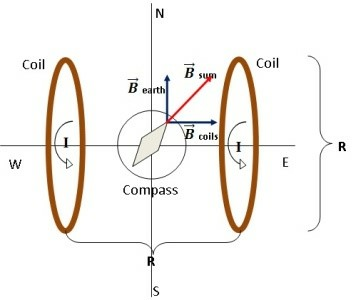
\includegraphics[scale=0.7]{compass}
    \caption{Disegno schematico delle due bobine viste dall'alto con il
    vettore di induzione magnetica generato dalle due bobine rispetto alla
    direzione Nord-Sud del campo magnetico terrestre
    \label{fig: compass}}
\end{figure}

Introducendo una terza bussola (quella di un telefono dotato di gps) si è
riusciti ad avere un risultato consistente, dato che le 2 bussole fornite non
erano in accordo tra loro (probabilmente per usura di una di queste)
per orientare l'apparato rispetto alla direzione di $B_T$.

\subsection{Mappatura del campo magnetico lungo l'asse delle bobine}
\label{sec:map}
Per caratterizzare il campo magnetico lungo il piano del moto degli elettroni
(il piano equidistante dalle 2 bobine) ne studiamo l'intensità al variare
della distanza dall'asse delle bobine.

Per farlo ci serviamo di una sonda ad effetto hall con fattore di conversione
di $\rho = 5.0 \pm 0.1 \; \si{m\V/G} = 50 \pm 1 \; \si{\V/\tesla}$.

A partire da una misura iniziale della corrente di alimentazione delle
spire
\[
I\ped{coil} = 2.00 \pm 0.03 \; \si{\A}
\]
tramite l'\cref{eq: Bmax} ci aspettiamo come massima intensità del campo
magnetico $B_{MAX} = 1.48 \pm 0.02 \; \si{m\tesla}$.

Per cui il solo sensore Hall non è sufficientemente sensibile alle variazioni
del campo magnetico (il sensore produrrebbe una d.d.p di circa 70 mV in
corrispondenza di $B_{MAX}$).
Si inserisce quindi tra la sonda e il multimetro un amplificatore-sottrattore
con un coefficiente di amplificazione pari a $G = 11.1 \pm 0.1$, per cui
facciamo riferimento all'equazione
\begin{equation}
B = \frac{\Delta V}{G \rho}
\end{equation}
per convertire il valore letto dal multimetro ($\Delta V$) in unità di campo
magnetico (nel resto della trattazione useremo i Tesla, ricordando che
$1 \; \si{G} = 10^{-4} \; \si{\tesla}$).

Dato che l'incertezza sulla lettura del multimetro risulta (da datasheet) pari
a $0.7 \percent + 1 \; \si{digit}$ rispetto al contributo del
$2 \percent \oplus 1 \percent$ derivante dal circuito sonda + amplificatore,
non ne teniamo in considerazione nella stima dell'incertezza associata alle
misure di $\Delta V$.

Calibrare il circuito amplificatore-sottrattore aggiustando l'offset non è
banale, essendo presente un campo magnetico residuo non si può semplicemente
cambiare la resistenza del potenziometro finché il valore letto sul multimetro
si annulli (così staremo solamente ponendo l'offset pari al valore in
ingresso al sottrattore).

Di conseguenza abbiamo aggiustato l'offset in modo che dal multimetro si
leggessero 2 valori di modulo uguale (compatibili entro l'incertezza) ma
segno opposto ruotando la sonda di $180 \degree$, cioè misurando in verso
opposto lo stesso campo d'induzione magnetica.

La sonda viene inserita nella guida rettilinea posta nel punto medio tra le
due bobine e passante per il loro centro, orientando quindi il sensore nella
direzione perpendicolare all'asse del campo magnetico generato.
Ad alimentazione spenta misuriamo una tensione di
${\Delta V}_0 = 19.0 \pm 0.2 \; \si{m\V}$, corrispondente ad un campo magnetico
di $B_0 = 34.2 \pm 0.7 \; \si{\micro \tesla}$, compatibile con l'intensità del
campo magnetico terrestre (riportata da Wikipedia) $B_T \in [25, 65] \;
\si{\micro\tesla})$.

Notiamo che questo contributo non risulta trascurabile rispetto all'incertezza
associata a $B_{MAX}$, per cui ci aspettiamo che il campo magnetico misurato
risulti maggiore di circa un $2 \percent$, rendendo la nuova aspettativa di
$B_{MAX} = 1.51 \pm 0.02 \; \si{m\tesla}$.

Quindi, una volta alimentate le bobine con la stessa $I\ped{coil}$ di prima,
abbiamo registrato le misure di intensità del campo generato ottenute dal
multimetro all'avanzare della sonda lungo la guida a passi regolari di circa
un centimetro, che riportiamo in \cref{fig: Bpos}.

\begin{figure}[htbp]
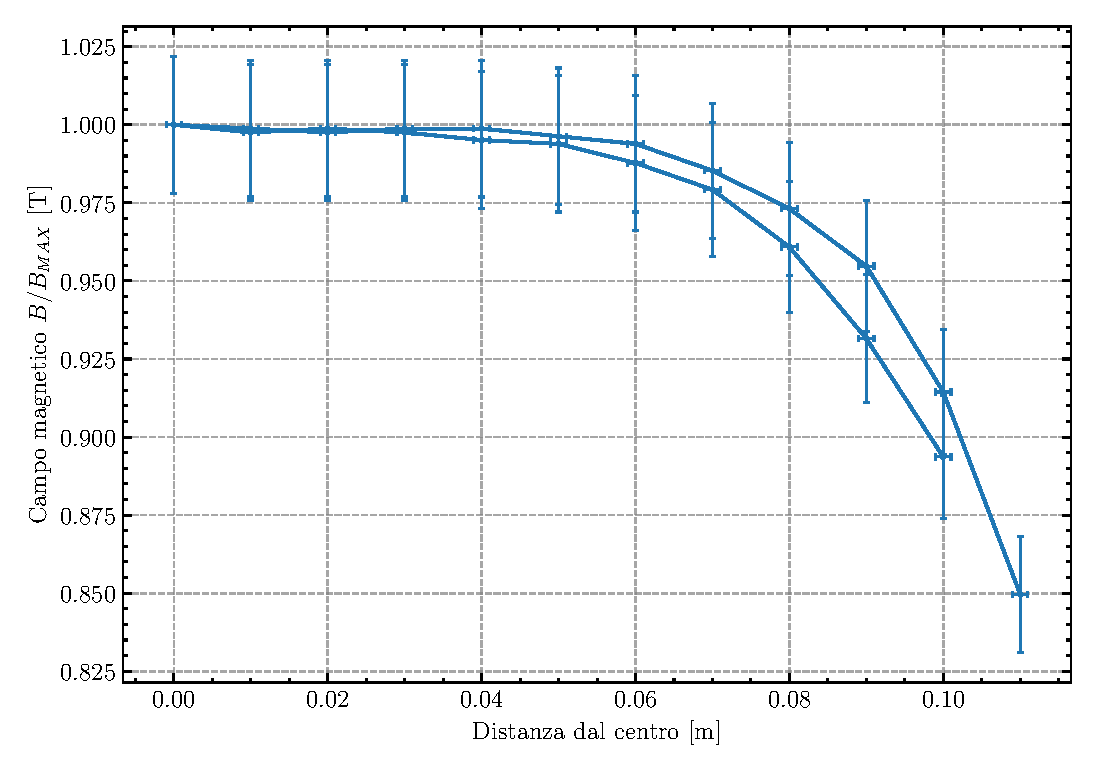
\includegraphics[width=\textwidth]{Bdist}
\caption{Andamento misurato dell'intensità del campo magnetico a metà tra le
spire al variare della distanza dall'asse. \label{fig: Bpos}}
\end{figure}

Il campo magnetico generato dalle bobine in realtà non è uniforme, ma presenta
una dipendenza sia dalla distanza dall'asse $r$ che dalla distanza dalle
bobine lungo l'asse $z$, completamente trascurata nel nostro modello.

Confrontando il grafico teorico per $B_z(r)$ in \cref{fig: Bref} normalizzato
rispetto al valore massimo troviamo che la nostra mappatura del campo risulta
quantomeno qualitativamente compatibile con il suo andamento atteso.
\begin{figure}[htbp]
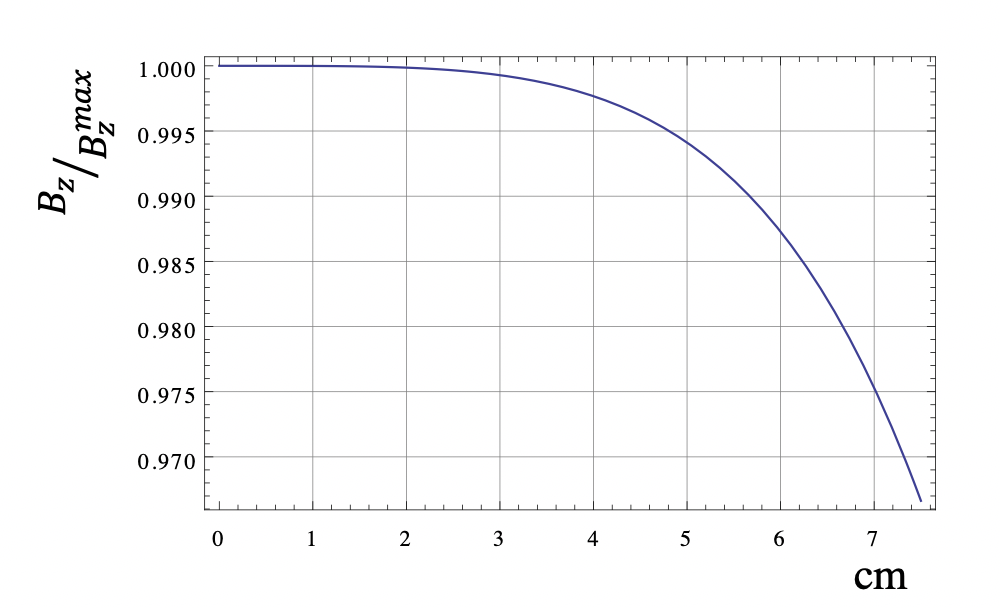
\includegraphics[width=\textwidth]{riferimentoB}
\caption{Andamento previsto per l'intensità del campo magnetico nel piano
centrale tra le spire in funzione della distanza dal centro \label{fig: Bref}}
\end{figure}

Notiamo esplicitamente come l'intensità del campo magnetico risulta essere
costante (entro la sensibilità sperimentale) all'interno della zona che sarà
poi occupata dal bulbo (che consideriamo come una sfera di raggio
$R\ped{bulb} \approx 7 \; \si{c\m}$ con centro posto all'intersezione tra
l'asse delle spire e il piano equidistante tra le medesime).

Osserviamo infine che la massima intensità del campo magnetico misurata,
trovata in corrispondenza del centro delle spire, è pari a
$B_{MAX} = 1.47 \pm 0.03 \; \si{m\tesla}$, risultato compatibile con le
aspettative entro l'incertezza.

\subsection{Calibrazione dell'apparato per l'acquisizione delle traiettorie}
Si è posizionata la fotocamera in modo tale che l'asse centrale
dell'obiettivo coincidesse con il centro della sfera di vetro, così da
minimizzare gli effetti di distorsione introdotti dalla rifrazione del bulbo
(ci aspettiamo che un fascio di luce proveniente dal centro della sfera non
subisca alcuna deviazione in uscita) sulla misura del raggio effettivo delle
orbite.

Abbiamo prima scattato una foto (riportata in \cref{fig: cal}) senza bulbo
in cui si vedono i due righelli (risoluzione 1 mm) posizionati davanti ad una
bobina ciascuno, per valutare gli effetti della geometria proiettiva, quindi
ottenere un fattore di conversione pixel-cm.
\begin{figure}[htbp]
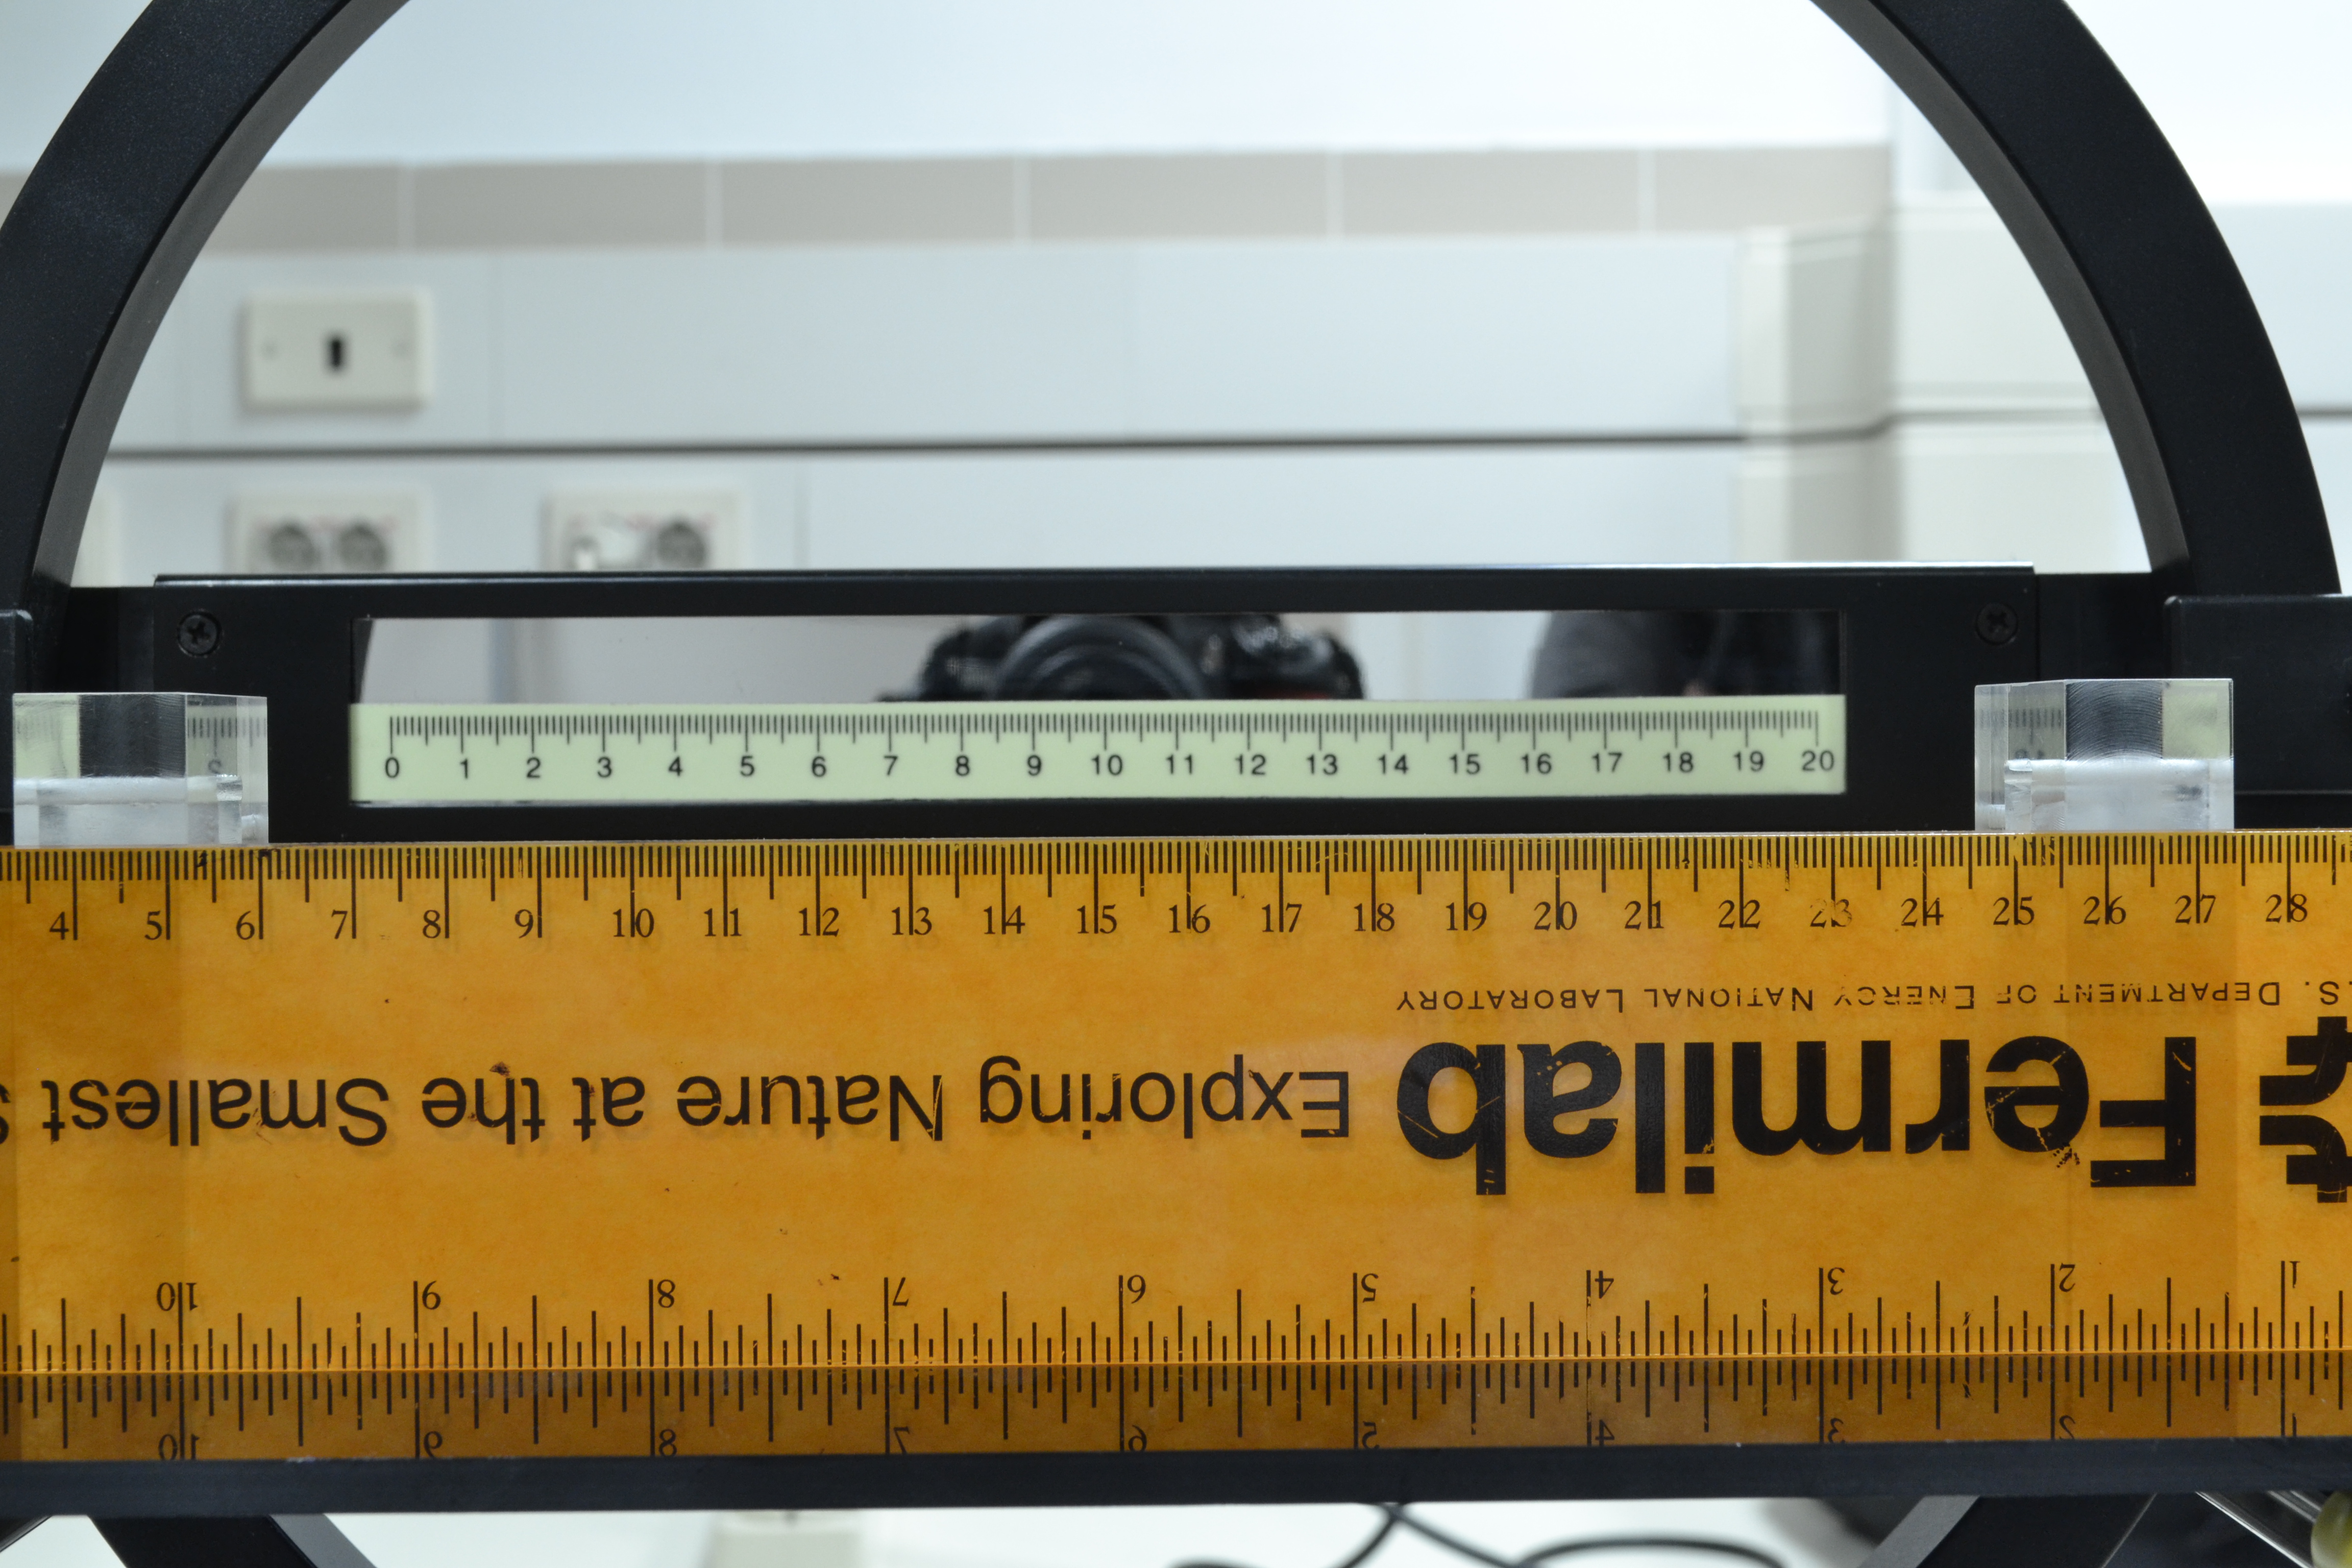
\includegraphics[width=\textwidth]{cal1}
\caption{Foto di calibrazione in assenza di bulbo da cui si ricava il fattore
di conversione per i dati da pixel a cm \label{fig: cal}}
\end{figure}

Dunque se ne scatta una seconda, stavolta con il bulbo inserito, per dare una
stima dell'ordine di grandezza atteso per gli effetti di distorsione del
bulbo.

Una volta alimentato il dispositivo di emissione di elettroni con una tensione
di $6 \; \si{\V}$ e atteso il tempo necessario affinché il filamento si
scaldasse fino a raggiungere la temperatura ottimale per cui il pennello
elettronico diventa chiaramente visibile si è iniziata la presa dati.

Si sono scattate cioè diverse fotografie al variare della tensione di
accelerazione $V\ped{acc}$ e intensità di corrente $I_{coil}$, sempre facendo
in modo che la traiettoria risultasse circolare e che il fascio di elettroni
non venisse deviato dal vetro. Come ci si aspettava, aumentando $V\ped{acc}$
aumenta il raggio di curvatura, mentre aumentando $I_{coil}$ (quindi
l'intensità del campo magnetico) il raggio dell'orbita si restringe.

Come impostazioni per la fotocamera abbiamo utilizzato un ISO di 400 e
un tempo di esposizione di 10 secondi, per distinguere al meglio i limiti
interni ed esterni del pennello elettronico, mantenendo la macchina fotografica
nella stessa posizione rispetto all'apparato, in modo da poter applicare lo
stesso fattore di scala pixel-cm per tutte le misure così effettuate.

\subsection{Conversione pixel-unità di lunghezza}
\label{sec: conv}
Se individuiamo un cono visivo per la fotocamera, diciamo che questo individua
sul righello della bobina più vicina la distanza $x$ e su quello più lontano
una distanza $y$ (in blu), possiamo stimare il rapporto $x/y$ confrontando le
scale graduate dei righelli fotografati in \ref{fig: cal}.
Chiamiamo allora $D_x$, $D_y$, $D_{xy}$ le distanze dalla fotocamera ai/tra i
vari piani e $D_{xe}$ la distanza tra il primo righello $x$ e il piano del
moto degli elettroni come nello schema in \ref{fig: conversione}

Allora per similitudine deve valere che
\[
\frac{y}{x} =
\frac{D_y}{D_x} = 1 + \frac{D_{xy}}{D_x}
.\]
Da cui troviamo una relazione tra il raggio misurato dal righello sul retro
($y$) e il raggio reale della traiettoria:
\[
    R = R_y \frac{D_x + D_{xe}}{D_x + D_{xy}} =
    R_y \left[\frac{D_{xe}}{D_{xy}} +
    \frac{x}{y} \left(1 - \frac{D_{xe}}{D_{xy}}\right) \right] = \gamma R_{y}.
\]

Detto $\eta$ il fattore di conversione tra pixel e i centimetri del righello
$y$, abbiamo
\[
R \; [\si{\centi\meter}] = \frac{\gamma}{\eta} R_y [\mathrm{px}]
.\]

Dalle misure riportate nella scheda dell'esperienza si ottiene, associando
un'incertezza di $\SI{1}{\milli\meter}$ a tutte le lunghezze appena definite
\begin{align*}
\gamma &= (906 \pm 5) \times 10^{-3} \\ 
\eta &= 141 \pm 6
\end{align*}

\begin{figure}[htbp]
    \centering
    \includesvg[width=\textwidth]{geometria}
    \caption{\label{fig: conversione} Schema geometrico dell'apparato di
    misura usato per la conversione px $\to$ cm e per la correzione
    degli effetti di geometria proiettiva.}
\end{figure}

\subsection{Misura del raggio della traiettoria}
Sulle foto acquisite come sopra si è effettuato un campionamento dei punti
sull'arco interno e sull'arco esterno delle traiettorie (dato che il pennello
elettronico ha uno spessore non trascurabile). Le coordinate dei pixel così
ricavate sono state interpolate con un \emph{fit} circolare per ottenere una
stima dei raggi di curvatura.

Si è effettuato sulle stesse prese dati un fit ellittico; in tutte le
fotografie i due semiassi risultano compatibili tra loro, quindi
prendiamo come miglior stima del raggio quello ricavato dal fit circolare

Durante il campionamento dei punti abbiamo osservato come la metà destra
della traiettoria ``circolare'' sia leggermente deviata verso il cannone
di elettroni, per cui si è scelto di considerare nel fit solamente i punti
lungo la prima metà della traiettoria (quindi solo il semicerchio sinistro
compiuto dagli elettroni appena emessi, come visibile in \cref{fig: circfit}
e nella fotografia originale \cref{fig: fot}).
\begin{figure}[htbp]
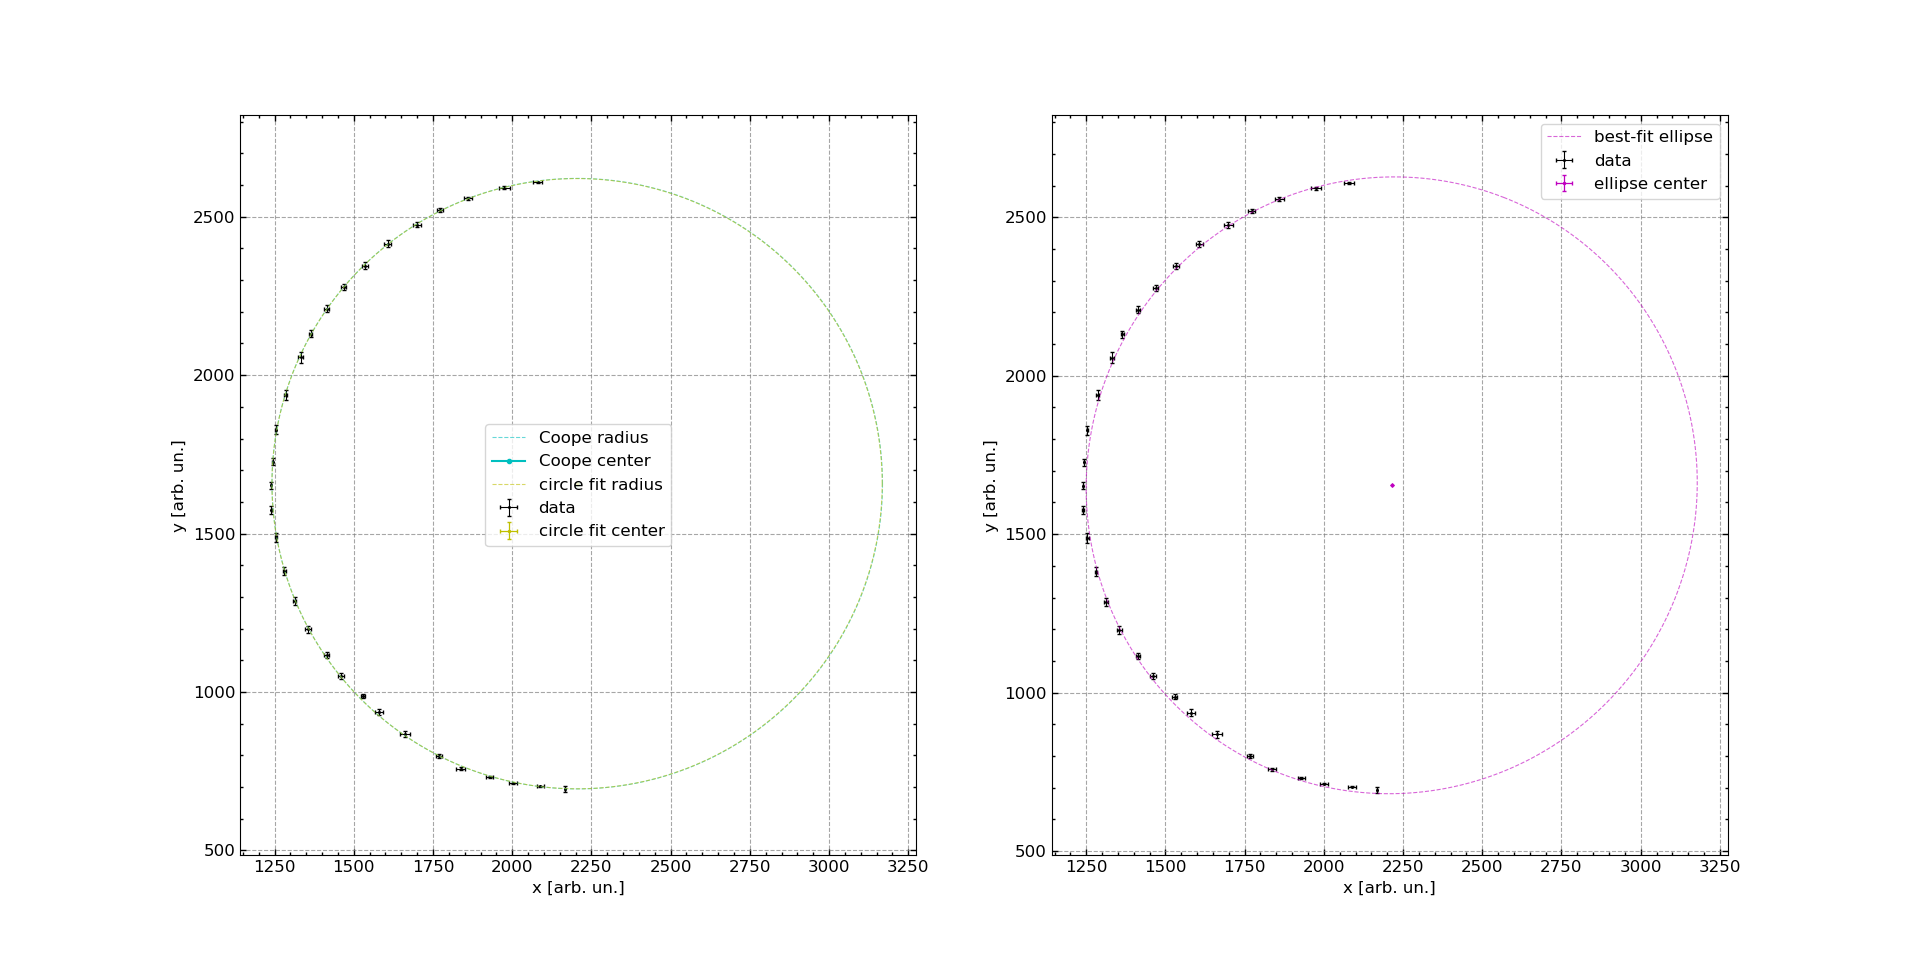
\includegraphics[width=\textwidth]{circfit}
\caption{Grafico del fit circolare (ed ellittico) dei punti acquisiti, in
questo caso rappresentanti l'orbita interna degli elettroni per la fotografia
con $V\ped{acc} = 290 \; \si{V}$ e $I\ped{coil} = 1.40 \pm 0.02 \si{A}$.
\label{fig: circfit}}
\end{figure}

\begin{figure}[htbp]
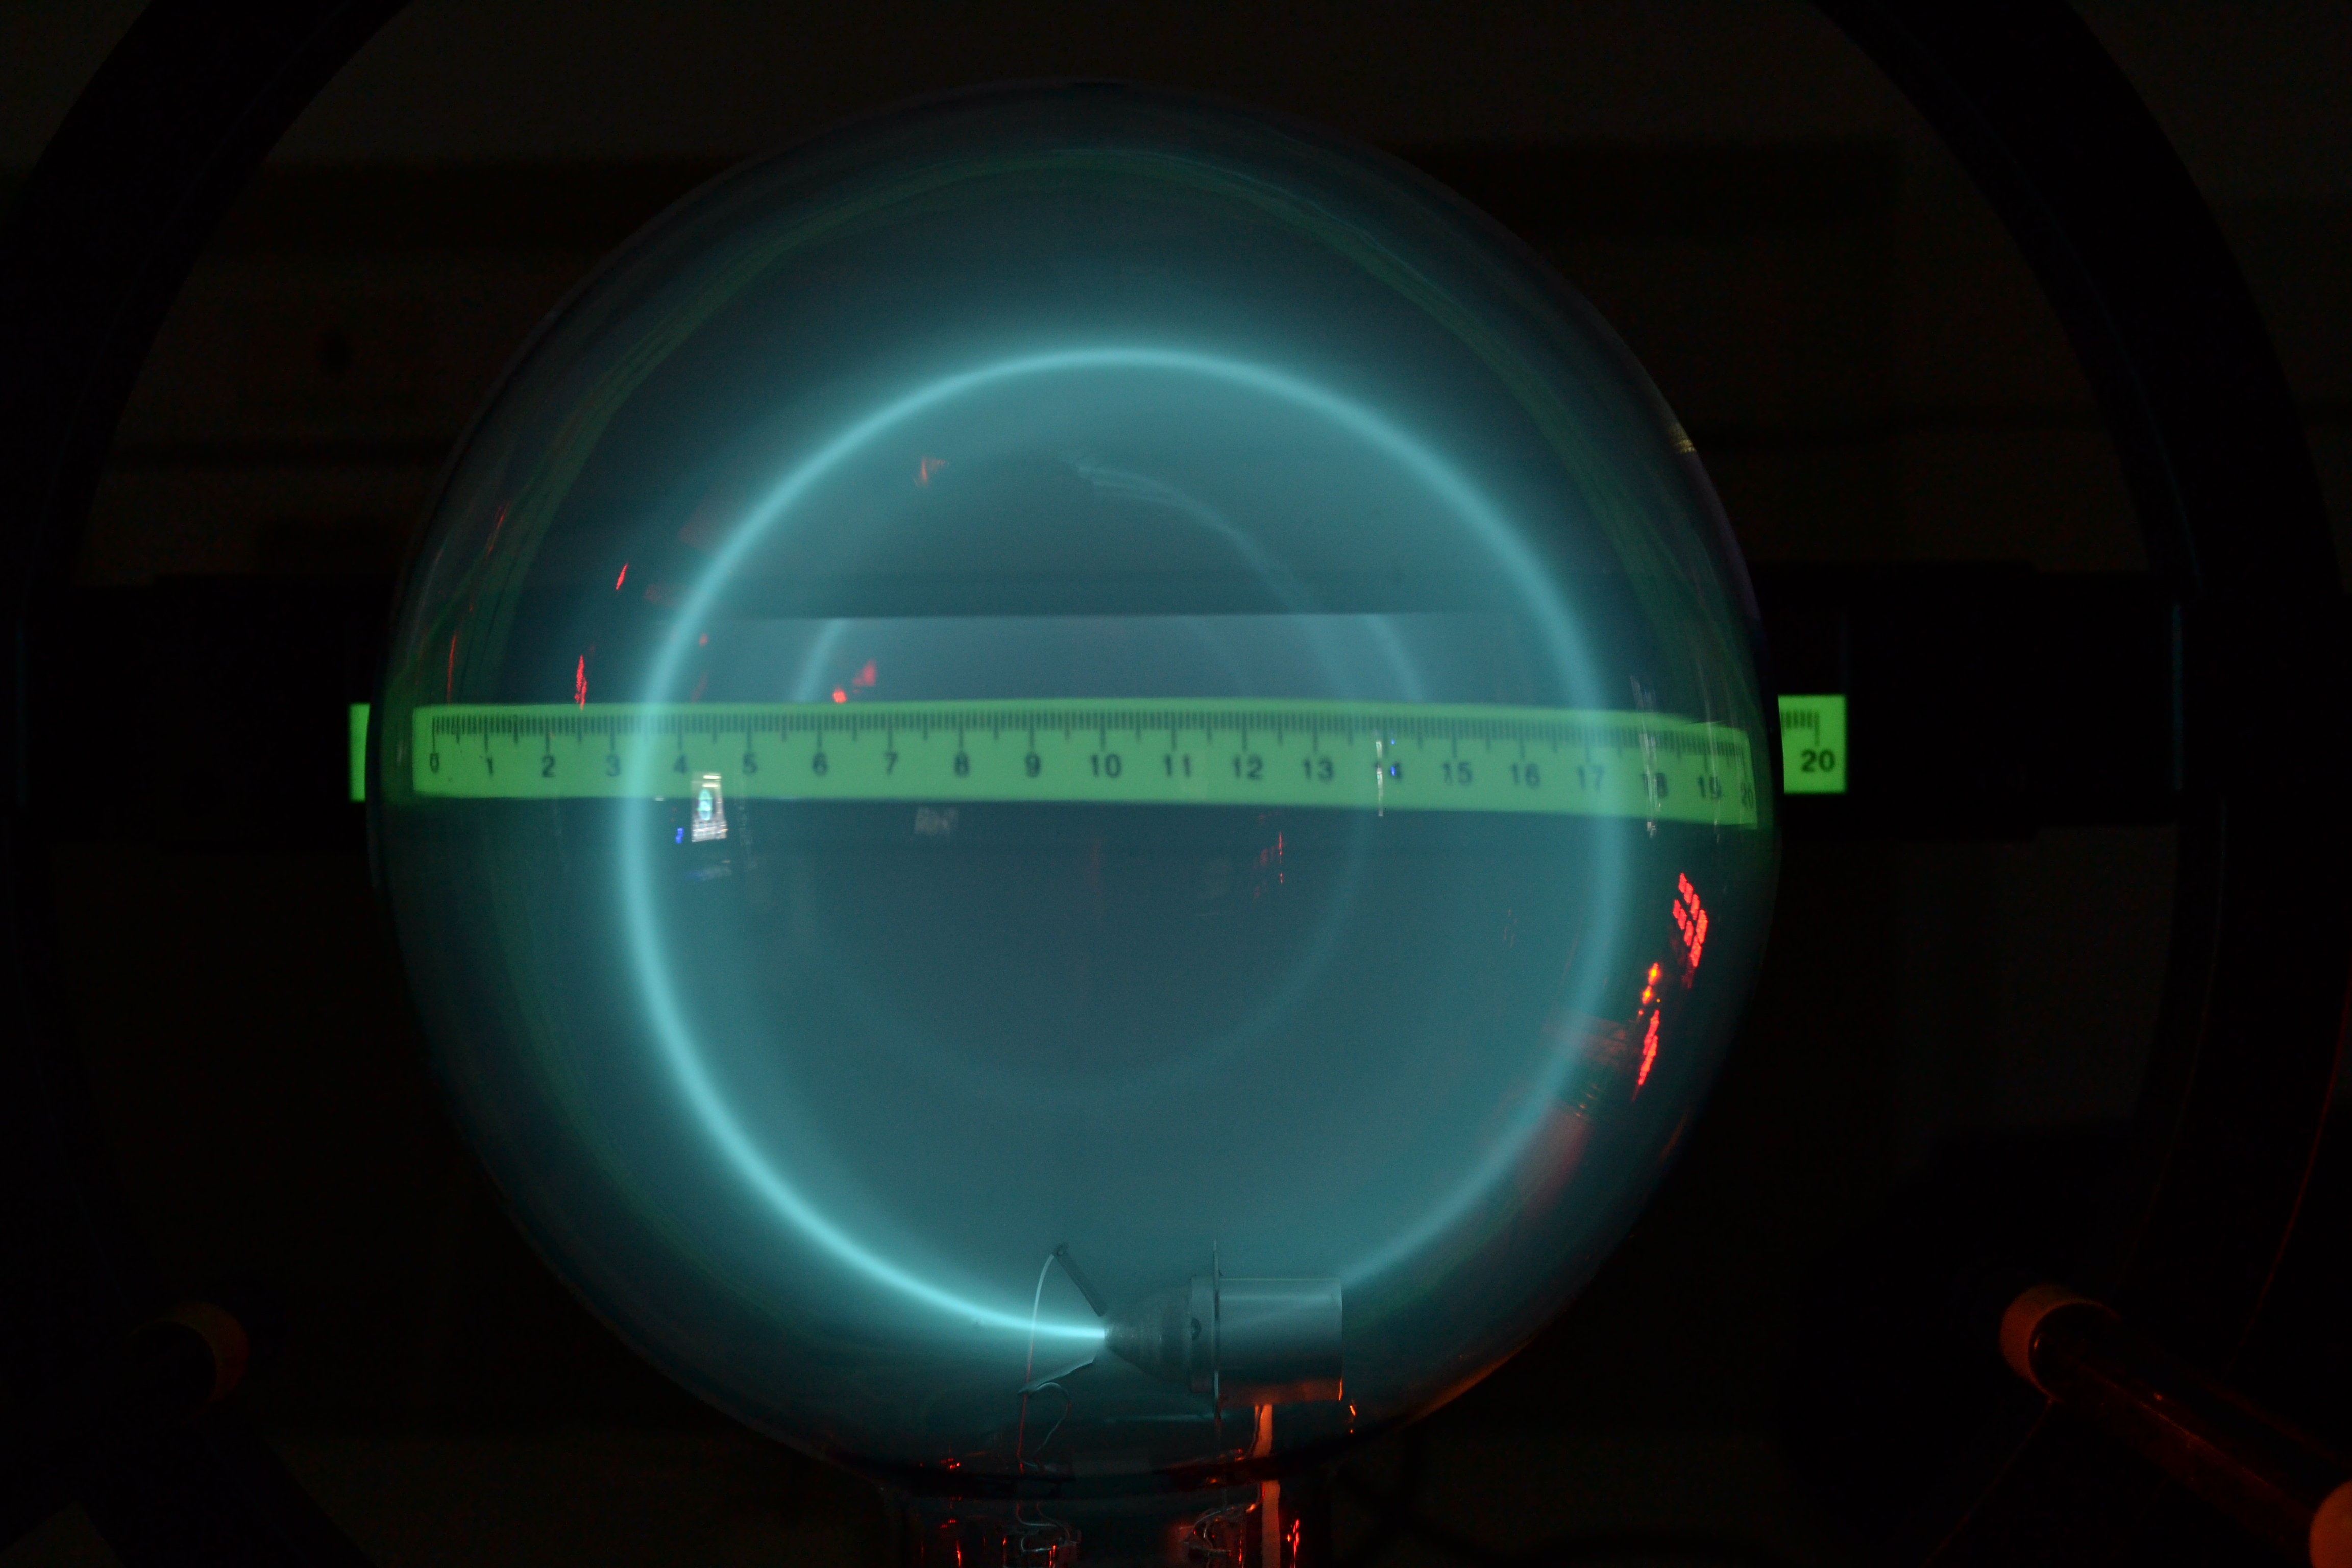
\includegraphics[width=\textwidth]{DSC_0120}
\caption{Fotografia dell'apparato sperimentale con $V\ped{acc} = 290 \; \si{V}$
e $I\ped{coil} = 1.40 \pm 0.02 \si{A}$.
\label{fig: fot}}
\end{figure}
Scegliamo di prendere come stima ottimale del raggio delle orbite la
media del raggio del cerchio interno e di quello esterno, a cui si associa
un'incertezza pari alla semi-dispersione tra i due valori estremi.

Le misure dei raggi sono state finalmente convertite in unità fisiche secondo
quanto illustrato nella ~ \cref{sec: conv}, ne riportiamo in
\cref{tab: IVrad} i valori trovati al variare della tensione di accelerazione.
\begin{table}[htbp]
\centering
\begin{tabular}{cc|c}
\toprule
$\Delta V_{acc} \; [\si{V}]$ & Raggio $[\si{cm}]$ & $I_{coil} [A]$ \\
\midrule
$150 \pm 1$ & $4.2 \pm 0.3$ & $1.40 \pm 0.02$\\
$170 \pm 1$ & $4.5 \pm 0.3$ & \\
$190 \pm 1$ & $4.8 \pm 0.3$ & \\
$210 \pm 1$ & $5.0 \pm 0.3$ & \\
$230 \pm 1$ & $5.2 \pm 0.3$ & \\
$250 \pm 1$ & $5.5 \pm 0.3$ & \\
$270 \pm 1$ & $5.7 \pm 0.3$ & \\
$290 \pm 1$ & $5.9 \pm 0.3$ & \\
\bottomrule
\end{tabular}
\caption{Misure dei raggi estrapolati dalle traiettorie in funzione delle
tensioni di accelerazione mantenendo $I\ped{coil}$ fissa.
\label{tab: IVrad}}
\end{table}

\section{Analisi dati e stima del rapporto $e/m$}
Prendendo come valori esatti $e = 1.602176634 \times 10^{-19} \; \si{\coulomb}$
e $m_{e} = 9.10938370 \times 10^{-31} \; \si{\kilogram}$ il valore atteso per
il loro rapporto è
\begin{equation}\label{eq: e-m-exp}
\left(\frac{e}{m_e}\right)\ped{exp} =
1.76 \times 10^{11}\; \si{\coulomb/\kilogram}
\end{equation}

Una prima stima del rapporto $e/m_e$ si è ottenuta come media pesata delle
singole misure ottenute dalla~\cref{eq: fit} e \cref{eq: Bmax}, che risulta
pari a
\[
\frac{e}{m_e} = 1.55 \pm 0.07 \; \times 10^{11} \; \si{\coulomb/\kilogram}
\]

Si inoltre effettuato un fit lineare usando come modello la funzione
\[
(BR)^2 = \frac{m_e}{e} 2 V\ped{acc} + q
\]
di modo che le incertezze sulle ascisse ($2 V\ped{acc}$) opportunamente
propagate fossero trascurabili rispetto a quelle sulle ordinate (${BR}^2$)
i cui risultati sono riassunti in \cref{tab: linfit} e \cref{fig: linfit}.
\begin{table}
\centering
\begin{tabular}{ccccc}
\toprule
$\m_e/e$ [kg/C] & $q$ [$\si{\tesla^2 m^2}$] & $\chi^2/\text{ndof}$ & norm. cov. \\
\midrule
$(152 \pm 3) \; \times 10^{9}$ & $(-6 \pm 5) \; \times 10^{-11}$ &
$0.1/6$ & $-0.98$ \\
\bottomrule
\end{tabular}
\caption{Risultati del fit lineare per la misura del rapporto $e/m_e$
\label{tab: linfit}}
\end{table}

Dal reciproco del coefficiente della retta di best-fit si trova un valore del
rapporto
\[
\frac{e}{m_e} = 1.52 \pm 0.03 \; \times 10^{11} \; \si{\coulomb/\kilogram}
\]

\begin{figure}
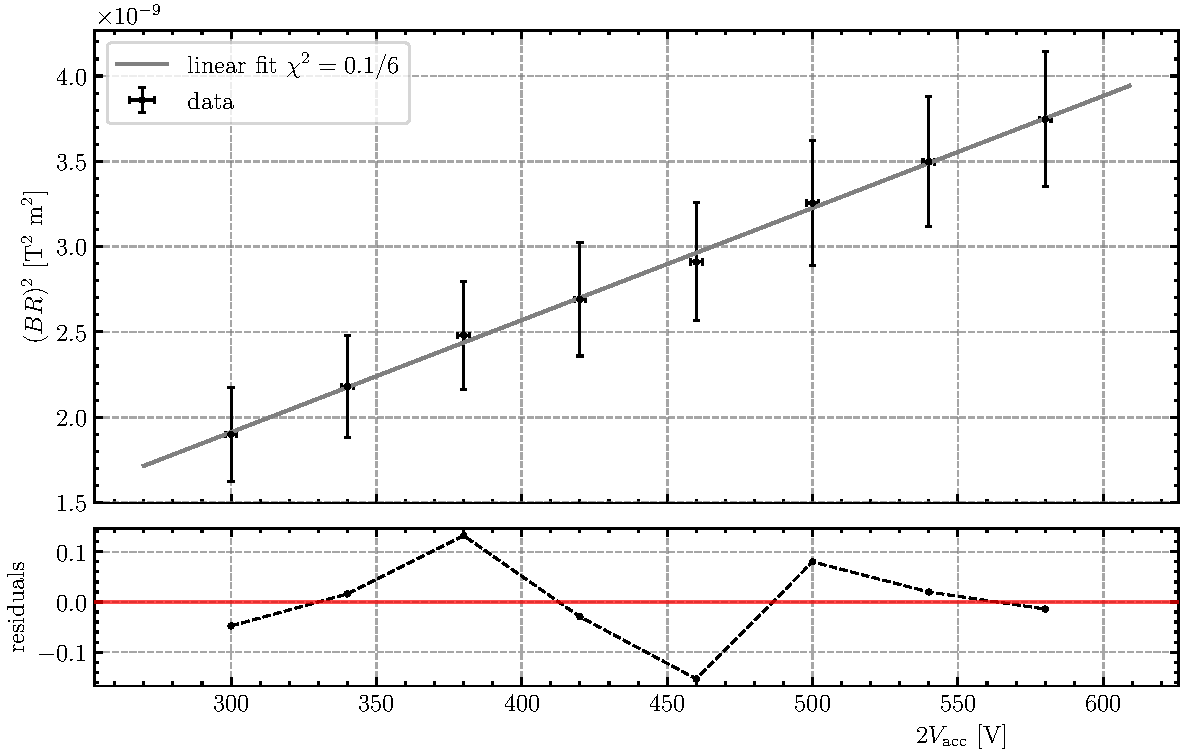
\includegraphics[width=\textwidth]{lin}
\caption{Grafico e residui del fit lineare in cui come modello è stata scelta
quella una retta di coefficiente angolare $\frac{m}{e}$.
\label{fig: linfit}}
\end{figure}

Né dal grafico dei residui del fit lineare in \cref{fig: linfit}, né dal
grafico dell'andamento della media pesata al variare di $V\ped{acc}$ (in
\cref{fig: medpes}) si riesce ad apprezzare una dipendenza della stima del
rapporto $e/m_e$ dal raggio della traiettoria degli elettroni.

\begin{figure}
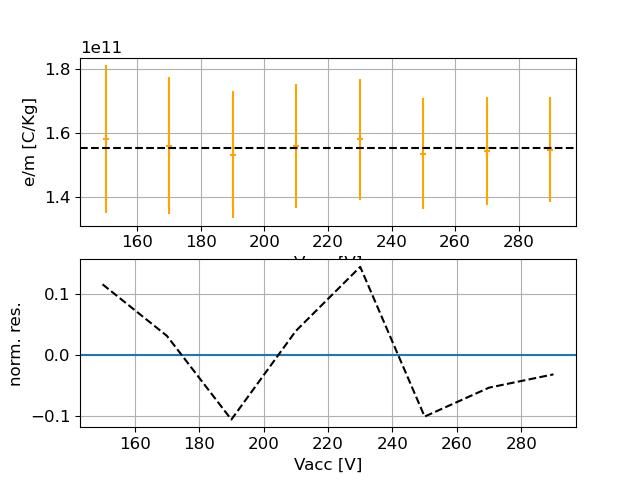
\includegraphics[width=\textwidth]{medpes}
\caption{Grafico e residui della media pesata sulle singole misure di $e/m_e$
\label{fig: medpes}}
\end{figure}

Le misure del rapporto $\frac{e}{m_e}$ ottenute dalle due procedure risultano
compatibili tra di loro, ma distanti dal valore atteso con uno scarto del
$14 \percent$ circa. 

%=======================
\section{Valutazione degli effetti sistematici}

\subsection{Spessore del pennello elettronico}
Un fattore che gioca un ruolo importante nella stima del raggio è lo spessore
del pennello elettronico: quest'ultimo infatti ha uno spessore di circa 20
pixel già a partire dal cannone elettronico (prendendo lo spessore in un
punto successivo della traiettoria è ancora più grande) che corrisponde
a 1.4 mm. Per poter prendere le misure al meglio abbiamo diminuito l'ISO
della fotocamera e aumentato il tempo di esposizione in modo che il raggio
interno ed esterno del pennello (in pratica i punti che delimitano la parte
più luminosa) fossero facilmente riconoscibili in qualunque punto della
traiettoria. Dopodiché abbiamo fatto una media tra i raggi delle circonferenze che si trovavano singolarmente ed abbiamo utilizzato quel valore come raggio effettivo della traiettoria, e come incertezza abbiamo calcolato la loro semi-dispersione attorno alla media.

\subsection{Distorsione del bulbo di vetro}
Dato che abbiamo posizionato la fotocamera allineata col centro del bulbo, ci si aspettava che il fit lineare evidenziasse una dipendenza del rapporto $e/m$ in funzione del raggio dell'orbita: questo perchè aumentando il raggio aumentava il numero di punti presenti nella zona di distorsione massima (quelli più lontani dal centro dell'ampolla; la zona di minima distorsione è invece quella più vicina al centro), andando così a compromettere il valore del raggio ricavato.
Dal grafico dei residui del fit lineare invece notiamo che i residui dei singoli punti sono distribuiti casualmente attorno al modello, per cui anche se la distorsione è presente, non influenza i dati a tal punto da produrre deviazioni sistematiche apprezzabili.

\subsection{Campo magnetico terrestre}
Assumendo che gli unici contributi al campo magnetico totale derivino dalle bobine e dal campo magnetico terrestre, abbiamo orientato le bobine in modo che la direzione del campo magnetico generato e quello terrestre coincidessero
Abbiamo fatto particolare attenzione anche al verso della corrente, in modo che sia direzione che verso dei due campi coincidessero; il modulo del campo magnetico totale è quindi dato dalla somma delle 2 intensità.
Avendo misurato il valore dell'intensità del campo magnetico terrestre abbiamo notato che non risulta essere trascurabile rispetto al valore dell'intensità di quello generato essendo maggiore della sua incertezza; di conseguenza durante l'analisi dati abbiamo considerato come campo magnetico totale:
\[
B\ped{tot} = B_z + B_T
\]

\subsection{Disuniformità del campo magnetico sulla traiettoria}
A partire da quanto in \ref{sec:map} e dalla dimensione del bulbo di vetro possiamo affermare che finché la traiettoria rientra all'interno dell'area compresa entro i 7 cm dal centro del bulbo, la disuniformità del campo magnetico è tale da poter essere trascurata, essendo una variazione compresa all'interno dell'incertezza del valore d'intensità massima.
Dai datasheet reperibili online si trova che il diametro del bulbo è pari a 15.5 cm, e considerando le dimensioni e la posizione del cannone elettronico, possiamo affermare che tutte le traiettorie da noi analizzate sono comprese entro l'area con variazione di intensità del campo magnetico non apprezzabile e compresa nel valore dell'incertezza.

%=======================
\section*{Conclusioni e commenti finali}
Si è riusciti a dare una misura ragionevole del rapporto carica/massa
dell'elettrone a partire da un'analisi delle fotografie della sua traiettoria
in presenza di un campo magnetico uniforme, nonostante le diverse fonti di
incertezza sistematica che caratterizzano il metodo sperimentale utilizzato.

%=======================
\section*{Dichiarazione}
I firmatari di questa relazione dichiarano che il contenuto della relazione \`e
originale, con misure effettuate dai membri del gruppo, e che tutti i firmatari
hanno contribuito alla elaborazione della relazione stessa.

%=======================
\begin{thebibliography}{1}
\bibitem{Coope}{I. D. Coope, Circle fitting by linear and nonlinear least
squares, Department of Mathematics, University of Canterbury, Christchurch,
New Zealand, N.60, May, 1992,
\url{https://ir.canterbury.ac.nz/bitstream/handle/10092/11104/coope_report_no69_1992.pdf?sequence=1&isAllowed=y}}
\end{thebibliography}

\end{document}
